\providecommand*{\lstnumberautorefname}{line}

Reliability and productivity are challenging issues
currently effecting the design of VLSI/FPGA systems as
device density increases.
Addressing the latter issue High Level Synthesis (HLS) tools \cite{canis2011legup} have
been both commercially and academically successful at trading
performance for productivity, however their generated circuits are not reliable.
To generate reliable circuits engineers are often faced with either:
full circuit replication, which can be easily automated with tools but
is expensive in resource or power costs; or expend considerable
effort manually designing a reliable circuit.
%An easy approach to protecting circuits and increasing their reliability is to
%replicate the full circuit and compare the results.
%While this approach can be easily automated by tools
%it is often an infeasible due to power and resource costs
%required for full replication.

For reliable execution do we need full replication?
From reviewing the literature you would quickly discover the answer
is often application dependant but that for a significant number
there are distinct regions of critical and non-critical code,
especially in cases involving media processing or machine
learning\cite{wong2006soft} \cite{liu2012flikker}.
In this paper we argue that it is often the case that instructions important to the control flow of an application are more critical
than instructions that only effect data; for example, an image renderer which can tolerant errors within
it's pixel values but errors in it's control flow could cause it to hang indefinitely \cite{sampson2011enerj}.

%\subsection{Matrix Multiplication Example}
To demonstrate and highlight the potential saving that duplicating just
the control flow can achieve we will use an example of HLS circuit generated from a
matrix multiplication C function in \hyperref[lst:MMM]{Listing \ref{lst:MMM}}.
A representation of the generated circuit can be seen in Figure \ref{fig:singleHLSArch}
depicting the dataflow section containing functional units, and the
control FSM responsible for scheduling instruction execution on functional units.

\lstset{language=C}
\begin{lstlisting}[basicstyle=\ttfamily\footnotesize, frame=single, label={lst:MMM}, captionpos=b, caption={Matrix Multiplication Example},numbers=left,escapeinside={@}{@}]
void MMM(float A[5][5],float B[5][5],float C[5][5])
{ int i=0, j=0, k=0;
  for(i=0, i<5, i++){
    for(j=0, j<5; j++){
      C[i][j] = 0;
      for(k=0, k<5; k++){
        @\label{lst:MMM_2}@C[i][j] += A[i][k]*B[k][j]; }
    }
  }
}
\end{lstlisting}

\begin{figure}[h]
\centering
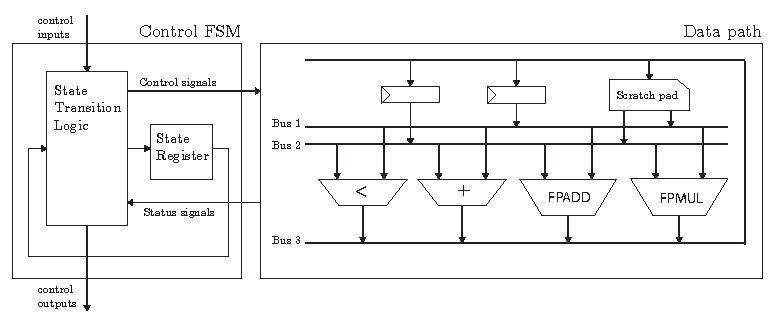
\includegraphics[width=3.5in]{./imgs/singleHLSArch.pdf}
\caption{Diagram representing a HLS circuit for the Matrix Multiplication example}
\label{fig:singleHLSArch}
\end{figure}
%The HLS generated circuit for this function can be divided into two main subsystems, a datapath, and a control FSM.
%Within the datapath are all the functional units required to perform the computation, which in our example will contain:
%integer comparators and incrementers for calculating the loop conditionals; and floating point adders and multipliers
%for computing line \autoref{lst:MMM_2} of Listing \ref{lst:MMM}.
%As the control FSM contains logic used for scheduling which operation is performed on a functional unit in the datapath,
%when that operation is performed, and how data is moved between functional units.

If this circuit was operating in the presence of soft errors then upsets within
the floating point addition and multiplication circuitry used to calculate line \ref{lst:MMM_2} could potentially cause the data in the output
matrix to be incorrect.
As errors in the integer functional units effecting lines 3,4 and 6
could cause the calculation of rows and columns of the output matrix \lstinline$C$ to be skipped, or even
worse, cause the circuit to enter an infinite loop and never terminate.

Let's say in this case errors in
the output are tolerable or can be detected through statistical means at a later point, but
there is a strict requirement that the circuit finishes in correct number of cycles and must
always terminates.
Initially we might try the industry standard of full circuit replication
but due to the expensive replication of the floating point units it is infeasible in both area and power.
Since we only need to ensure that the circuit takes the appropriate cycles,
we might try and duplicate just the control FSM however this wont work since state transitions
within the control FSM are dependant on the outputs of results in the datapath.
Eventually we realise that by removing the floating point units from the datapath
it is  possible to protect all the control decisions of the program while reducing the amount of resources required
to do so.

Manual inspecting code and removing elements that don't influence control flow
may be feasible in the simple case of Matrix Multiplication, however as the complexity of the input increases
the engineering effort required in both analysing the input source and generating circuits with an identical control FSM is
significant.
StitchUp fully automates this process through using a static analysis technique, known as program slicing, to extract
and duplicate any instructions that may influence control.

The contribution of this paper are:
\begin{itemize}
\item StitchUp, a tool which can automatically extract and protect the control flow structure of a circuit generated with a HLS tool.
\item Detailed results of the CHStone benchmark, where exhaustive fault injection is performed on the majority of circuits.
\item Results exploring the reliability of StitchUp protected circuits as the control to data ratio is varied through
loop unrolling in the matrix multiplication example.

\end{itemize}


%Can we automatically replicate system components at a very
%fine level of granularity, such as the level of assembly instructions?


%FPGAs are great but have problems
%FPGAs are an ideal candidate platform for aerospace and automotive applications
%when there are strict constraints on performance and power, yet they are seldom used.
%Two main issues prevent widespread adoption in these fields: firstly they are difficult
%to program with designs taking many man-hours to build and verify;
%and secondly they are highly susceptible to soft errors with single event upsets (SEU)
%potentially causing unwanted device reconfiguration.
%Research into High Level Synthesis (HLS) has been academically and commercially successful
%at addressing the development time issues. HLS tools transform a popular programming language, such as C,
%into a digital circuit replacing expensive specialised hardware engineers with software engineers.
%However to address the issue of managing soft errors replication of the circuit and comparison logic is required
%costing large amounts of additional resources and power, potentially causing the design to break constraints.
%
%%Overview of our work
%This paper presents StitchUp which extends the LegUp HLS tool \cite{canis2011legup} so that produced circuits are
%guaranteed to terminate (provided the input does) even in the presence of SEUs, while always consuming equal or less logic than full circuit duplication.
%In order to achieve this the tool determines the set of instructions required to make an exact duplicate of the Control
%Flow Graph (CFG) ignoring instructions which only effect the data flow, creating what we shall refer to as a \emph{CFG shadow} circuit.
%We argue that it is often the case that instructions which may influence the control flow of an application are more critical
%than instructions which never effect control; for example, an image renderer which can tolerant errors within
%it's pixel values but errors in it's control flow could cause it to hang indefinitely \cite{sampson2011enerj}.
%
%The tool has three distinct stages: an analysis stage statically examines the input source and extracts any instruction
%which potentially effects control; a CFG shadow generation stage consists of a modified LegUp backend
%which takes the output of the analysis stage along with a description of the original schedule to produce a CFG shadow circuit;
%finally a wrapper generation stage combines the original circuit, the CFG shadow circuit, and generates error detection logic;
%Using this approach we are able to show that for certain applications we can guarantee that the CFG
%is followed correctly, while consuming only 4\% of the resources required of standard Dual Modular Redundancy approaches.
%
%%Below LEO
%Until recently soft error concerns have primarily been contained within domains where
%devices are placed in harsh radioactive conditions, such as satellites in low earth orbit, however
%with shrinking device geometries this issue is set to become a problem for the entire
%industry\cite{ibe2010impact}.
%If terrestrial devices start to become increasingly effected by ground level radiation
%then managing such faults is incredibly important especially in safety critical applications, such
%as driverless cars.\\
%
%%Typical Approaches are expensive, if you want to make guarantees
%Protecting against soft errors is often achieved using N-Modular Redundancy, where N identical
%versions of the module are executed, their outputs are compared and any differences in the
%result indicate that a fault has occurred.


%We present a way to protect a subset of the circuit, while being able to make some guarantees


